\documentclass[11pt,a4paper]{scrartcl}
\usepackage[T1]{fontenc}
\usepackage[utf8]{inputenc}
%\usepackage[ngerman]{babel}
\usepackage[ngerman,english]{babel}
\selectlanguage{english}
\usepackage{microtype}
\usepackage{lmodern}
\usepackage{amsmath}
\usepackage{amsfonts}
\usepackage{amssymb}
\usepackage{enumerate}
\usepackage{graphicx}
\usepackage{listings}
\usepackage{color}
\usepackage{url}
\usepackage{multicol}
\usepackage{wrapfig}
\usepackage{amsmath}
\usepackage{tikz}
\usetikzlibrary{arrows}


\begin{document}

\author{Ralf Vogler}
\title{Program Optimization}
\subtitle{Exercise sheet 9}

\maketitle


\section*{Exercise 1: Inlining}
\subsection*{a) Call graphs}
\begin{tikzpicture}[->,>=stealth',shorten >=1pt,auto,node distance=1.8cm,
  thick,main node/.style={fill=blue!20,draw,font=\sffamily\Large\bfseries}]

  \node[main node] (1) {main};
  \node[main node] [below left of=1] (2) {add10};
  \node[main node] [below right of=1] (3) {decr};

  \path[every node/.style={font=\sffamily\small}]
    (1) edge node [left] {} (2)
    (1) edge node [right] {} (3)
    (3) edge [loop right] node [left] {} (3);
\end{tikzpicture}

\subsection*{b) Inline leaf-procedures}
\definecolor{dkgreen}{rgb}{0,0.6,0}
\lstset{
  numbers=left,                   % where to put the line-numbers
  numberstyle=\color{gray},  	  % the style that is used for the line-numbers
  numbersep=5pt,                  % how far the line-numbers are from the code
  keywordstyle=\color{blue},          % keyword style
  commentstyle=\color{dkgreen},       % comment style
}
\begin{lstlisting}[language=C]
main() {
	h=2;
	g=0;
	
	// initialize local variables of add10
	n=0;
	
	// begin of inlined add10
	n=10;
n12:	g=g+1;
	n=n+1;
	if(n>0) goto n12;
	// n15
	
	// end of inlined add10
	;
	
	decr();
_exit:
}
\end{lstlisting}

\subsection*{c) New call graphs, unreachable procedures}
\begin{tikzpicture}[->,>=stealth',shorten >=1pt,auto,node distance=1.8cm,
  thick,main node/.style={fill=blue!20,draw,font=\sffamily\Large\bfseries}]

  \node[main node] (1) {main};
  \node[main node] [below left of=1] (2) {add10};
  \node[main node] [below right of=1] (3) {decr};

  \path[every node/.style={font=\sffamily\small}]
    (1) edge node [right] {} (3)
    (3) edge [loop right] node [left] {} (3);
\end{tikzpicture}\\
The procedure verb|add10| is not reachable from verb|main|.


\section*{Exercise 2: Tail recursion}
\subsection*{a) Transformation T11}
T11 replaces the call of fact() in fact() (node 13 to 14) with a reset of the locals and a jump to the beginning of fact() (\verb|goto _f|).

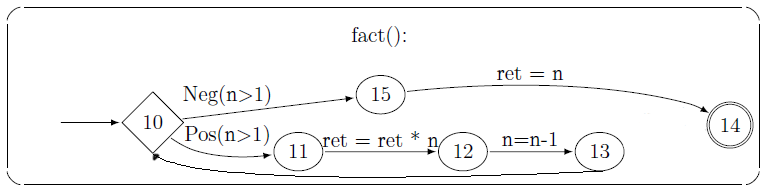
\includegraphics[scale=.5]{2_1}

\subsection*{b) Optimized main}
In the optimized version of main, the call to fact gets replaced by the definition of fact:

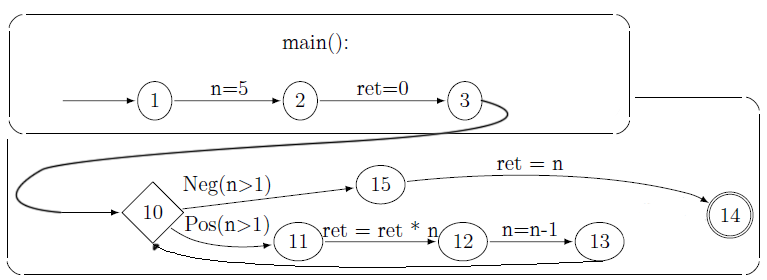
\includegraphics[scale=.5]{2_2}

% all: 521: werden globals in C wirklich erst mit dem combine, d.h. am Ende der Funktion geupdatet?
\section*{Exercise 3: Copy-Constant Analysis}
\subsection*{a) Copy-constant information}
\begin{minipage}[t]{0.5\textwidth}
main():\\
\begin{tabular}{|c|c|}
\hline
1 & $\{x \mapsto \top, y \mapsto \top\}$ \\
2 & $\{x \mapsto 0, y \mapsto \top\}$ \\
3 & $\{x \mapsto 0, y \mapsto 5\}$ \\
4 & $\{x \mapsto 5, y \mapsto 5\}$ \\
5 & $\{x \mapsto 5, y \mapsto \top\}$ \\
6 & $\{x \mapsto \top, y \mapsto \top\}$ \\
\hline
\end{tabular}
\end{minipage}
\begin{minipage}[t]{0.5\textwidth}
y2x():\\
\begin{tabular}{|c|c|}
\hline
11 & $\{x \mapsto \top, y \mapsto \top\}$ \\
12 & $\{x \mapsto y, y \mapsto \top\}$ \\
\hline
\end{tabular}
\end{minipage}
\subsection*{b) Reaching state information}
\begin{minipage}[t]{0.5\textwidth}
Constraints:\\
\begin{align*}
\mathcal{R}[1] &\sqsupseteq enter^\# d_0 \\
\mathcal{R}[2] &\sqsupseteq [x=0]^\# (\mathcal{R}[1]) \\
\mathcal{R}[3] &\sqsupseteq [y=5]^\# (\mathcal{R}[2]) \\
\mathcal{R}[11] &\sqsupseteq enter^\# (\mathcal{R}[3]) \\
\mathcal{R}[12] &\sqsupseteq [x=y]^\# (\mathcal{R}[11]) \\
\mathcal{R}[4] &\sqsupseteq [y2x()]^\# (\mathcal{R}[3]) \\
\mathcal{R}[5] &\sqsupseteq [y=x+5]^\# (\mathcal{R}[4]) \\
\mathcal{R}[11] &\sqsupseteq enter^\# (\mathcal{R}[5]) \\
\mathcal{R}[6] &\sqsupseteq [y2x()]^\# (\mathcal{R}[5]) \\
\end{align*}
\end{minipage}
\begin{minipage}[t]{0.5\textwidth}
Reaching definitions:\\
\begin{tabular}{|c|c|}
\hline
& $\mathcal{R}$ \\
\hline
1 & <x, 1>, <y, 1> \\
2 & <x, 2>, <y, 1> \\
3 & <x, 2>, <y, 3> \\
4 & <x, 4>, <y, 3> \\
5 & <x, 4>, <y, 5> \\
6 & <x, 6>, <y, 5> \\
\hline
\end{tabular}
\end{minipage}

\section*{Exercise 4: Sharir/Pnueli, Cousot}
y2x(): a = y, ret = x
\subsection*{a)}
$\{y \mapsto 5, x \mapsto 0\}$

\subsection*{b)}
$\{y \mapsto 5, x \mapsto 5\}$

\subsection*{c)}
$\{y \mapsto 10, x \mapsto 5\}$

\subsection*{d)}
$\{y \mapsto 10, x \mapsto 10\}$

\subsection*{e)}
$\{y \mapsto 10, x \mapsto 10\}$


\end{document}

















